\chapter{Parsing LL(1)}
\section{Introduzione}
Il parsing, o analisi sintattica, è una fase di compilazione  che viene utilizzata per definire la sintassi di un linguaggio di programmazione. In altre parole definisce la forma di un programma corretto. Utilizza i token [1], ossia sequenze di caratteri dotate di significato restituite da un analizzatore lessicale (Lexer); per produrre una rappresentazione intermedia ad albero che rappresenta la struttura grammaticale dei token. Una tipica rappresentazione è l'\textit{albero sintattico}, o \textit{syntax tree} in cui un nodo interno rappresenta un'operazione mentre i figli rappresentano gli argomenti dell'operazione; infine, questo albero prodotto, viene passato alle restanti fasi del processo di compilazione. In figura 1 viene mostrato il funzionamento del parser.
\par
\vspace{0.5cm}	
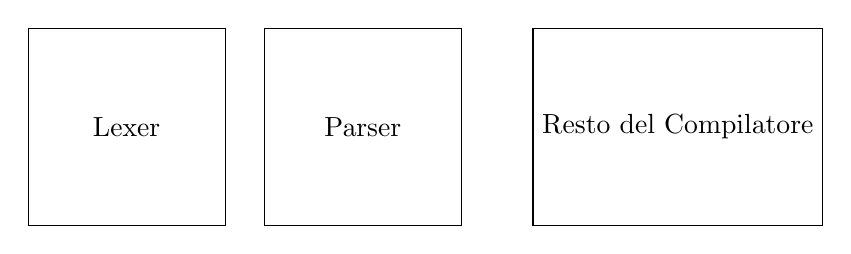
\begin{tikzpicture}
	\tikzset{every node/.style={draw, rectangle, minimum size=25mm}}
	%\draw [-latex, bend right] (Lexer) ;	
	\node (Lexer) at (0.0,2.5) {Lexer};
	\node (Parser) at (3.0,2.5) {Parser};
	\node (Resto) at (7,2.5) {Resto del Compilatore};
	\end{tikzpicture}
\section{Parsing top down}
%\subsection{paragrafo}
jrjfvrlf